\chapter{Term Indexing} \label{term_indexing}
In the following sections we give an overview of path indexing and discrimination trees. We also take a closer look at some details of their implementation in Isabelle/ML as they differ in many places significantly from the approaches chosen in most literature.

\section{Path Indexing}
A term can be represented as a tree with all symbols $s$ with $\arity (s) = 0$ as leafs and all functions $f(x_{1}, \dots, x_{n})$ as internal nodes with the $x_{i}$ as children. Within this tree, every symbol has a position determined by the nodes traversed to reach this symbol. We represent this as a sequence of $(symbol, index)$ pairs with the index describing which argument of a function is traversed. We call this sequence a path. The path of a symbol $s$ begins with the top symbol and ends with the index at which $s$ is located. For example, $\langle (f,2), (g,1) \rangle$ is the path of the symbol $a$ in $t = f(x,g(a,b))$. \Cref{termpaths} shows all the paths and symbols of $t$. We represent a path by enclosing the sequence of $(symbol, index)$ pairs with $\langle  \rangle$.

\begin{defn}
  A path is a sequence of $(symbol, index)$ pairs where the index describes the index of the next argument to traverse.\footnote{This is in contrast to coordinate indexing which only uses a sequence of indices \cite{noauthor_path-indexing_nodate}.} $Symbol_{t}(p)$ refers to the symbol associated with path $p$ in the term $t$.
\end{defn}

\begin{figure}[h]
\centering
\begin{tabular}{ c|l|l }
  Tree Representation & Path $p$ & $Symbol_t(p)$ \\
  \hline
\multirow{5}{4em}{\Tree [.f x [.g a b ] ]} & $\langle \rangle$ & $f$ \\
   & $\langle (f, 1) \rangle$ & $*$ \\
   & $\langle (f, 2) \rangle$ & $g$ \\
   & $\langle (f, 2), (g, 1) \rangle$ & $a$ \\
   & $\langle (f, 2), (g, 2) \rangle$ & $b$ \\
\end{tabular}
\caption{The paths and associated symbols of $t = f(x,g(a,b))$}\label{termpaths}
\end{figure}

A $(path, symbol)$ pair can be interpreted as a constraint on a term where at path $path$ there must be the symbol $symbol$. For example, the constraint $(\langle (f,1) \rangle, c)$ is only fulfilled by terms of the form $f(c,\dots)$. A term gives rise to a set of $(path, symbol)$ pairs, which, when interpreted as constraints, uniquely identify this term up to loss of variable identitification.

A term $t$ can either be represented by a set of paths and the $Symbol_{t}$ mapping or by listing each associated symbol explicitly in a set of $(path, symbol)$ pairs where $symbol = Symbol_{t}(path)$. We will choose whichever notation is clearer in the given context.

\subsection{Structure}
%The aforementioned constraints allow us to define terms not explicitly by their structure and symbols but rather by imposing constraints on them. This concept is fundamental to path indexing which stores only the constraints.
A path index builds on this idea of constraints and associates each $(path, symbol)$ pair with a set of terms that fulfill this constraint. For example, a path index storing the terms $\{f(x), f(a), g(a)\}$ will associate $(\langle \rangle, f)$ with the two terms $f(x)$ and $f(a)$.

\begin{defn}
  A path index is a function $index: Path \times Symbol \longrightarrow 2^{Term}$ that maps a constraint $(path,symbol)$ to the set of terms that fulfill this constraint and are stored in the path index.
\end{defn}

Storing the terms of $index$ such that it can be quickly evaluated for a $(path, symbol)$ pair can be achieved in multiple ways. We decided to use a prefix-sharing tree based approach as many of the paths share prefixes. The nodes of the tree contain a function $Terms_{p}: Symbol  \longrightarrow 2^{\T}$ where $p$ is the path from the root to the node. The edges are labelled with $(symbol, index)$ pairs, which correspond to the elements of a path.

\Cref{pathindex} shows a path index stored as a prefix-sharing tree. Note that we only use numbers to represent terms for better readability. The root contains a mapping from the symbol $f$ to all three terms as they all share this path. In the first argument, reached by the edge $(f,1)$, the symbol $a$ is mapped only to the first term whereas $*$ is mapped to the other two terms.

\begin{figure}[h]
  \begin{subfigure}{0.66\textwidth}
\begin{tikzpicture}[%every tree node/.style={draw,circle},
   level distance=2.25cm,sibling distance=1cm,
   edge from parent path={(\tikzparentnode) -- (\tikzchildnode)}]
\Tree
[.{$\{f \mapsto \{1,2,3\}\}$}
    \edge node[auto=right,pos=.6] {$(f,1)$};
    [.{$\{a \mapsto \{1\}, * \mapsto \{2,3\}\}$} ]
    \edge node[auto=left,pos=.6] {$(f,2)$};
    [.{$\{b \mapsto \{1,2\}, * \mapsto \{3\}\}$} ]
]
\end{tikzpicture}
  \end{subfigure}
  \begin{subfigure}{0.33\textwidth}
    \begin{tabular} { c|c }
      Index & Term\\
      \hline
      1 & $f(a,b)$\\
      2 & $f(x,b)$\\
      3 & $f(y,z)$
    \end{tabular}
  \end{subfigure}
  \caption{A path index storing three terms} \label{pathindex}
\end{figure}

When we insert a path $p$ of a term $t$, we start at the root and traverse the tree according to $p$. Once we reach the end of $p$ we extend $\terms_{p} (\sym_{t} (p))$ by $\{t\}$. To insert a term we simply insert all the paths that describe this term. This requires the insertion of many similar paths which benefits from the prefix sharing. Deleting a term $t$ is done almost identically. Instead of extending the $\terms_{p} (\sym_{t} (p))$ by $\{t\}$, we remove it.

\subsection{Queries}
Queries are answered by combining the different $\terms_{p}(s)$ sets with intersections or unions to retrieve a set of terms. For example, a $\var$ query for the term $t = f(x,g(a,b))$
procedes as follows:

\begin{enumerate}
  \item Compute the set of $(path, symbol)$ pairs describing the term.
  \item Retrieve the corresponding $Terms_{p}(s)$ from the index.
  \item Intersect the $Terms_{p}(s)$ to retrieve only the terms $u$ containing the same symbols at identical paths as the query term, that is, $Symbol_{t}(p) = Symbol_{u}(p)$
\end{enumerate}

Under the assumption of consistent typing, we retrieve only terms of identical structure as the query term. Due to the loss of variable identity we also retrieve variants of the query term in addition to the query term itself (if it is stored in the index).

To retrieve the unifiables of a term from the index, we can use some observations regarding the unification problem.
\begin{enumerate}
  \item A variable is unifiable with any other term
  \item Constants are unifiable with themselves and variables
  \item A function $f(x_{1},\dots,x_{n})$ is unifiable with term $t$ if and only if $t = x$ or $t = f(y_{1},\dots,y_{n})$ where, for all $i$, $x_{i}$ is unifiable with $y_{i}$.
\end{enumerate}

\newcommand{\PT}{terms_{p}}
\newcommand{\ALL}{AllTerms}
Using this, we can define an algorithm recursing on the structure of the query term while intersecting and unifying the different path sets of the index. \Cref{path_queries} shows the recursive definition for all the queries. As can be seen, the different queries are quite similar, with $\var$ being the most restrictive and $\unif$ the least restrictive. $\ALL$ is the set of all terms stored in the index and represents a wildcard at this path as intersecting $\ALL$ with an arbitrary $\PT$ returns $\PT$.

\begin{table}[h]
  \centering
\begin{adjustbox}{width=1\textwidth}
\begin{tabular}{ l|l|l|l }
  \diagbox{Query}{Arguments} & $Q(p, x)$ & $Q(p, a)$ & $Q(p, f(t_{1}, \dots, t_{n}))$ \\
  \hline
  $Q = \var$ & $\PT(*)$ & $\PT(a)$ & $\bigcap_{i} Q(\ang{p, (f, i)}, t_{i})$\\
  $Q = \ins$ & $\ALL$ & $\PT(a)$ & $\bigcap_{i} Q(\ang{p, (f, i)}, t_{i})$\\
  $Q = \gen$ & $\PT(*)$ & $\PT(a) \cup \PT(*)$ & $\bigcap_{i} Q(\ang{p, (f, i)}, t_{i}) \cup \PT(*)$\\
  $Q = \unif$ & $\ALL$ & $\PT(a) \cup \PT(*)$ & $\bigcap_{i} Q(\ang{p, (f, i)}, t_{i}) \cup \PT(*)$\\
\end{tabular}
\end{adjustbox}
\caption{The recursive definition of the queries}
\label{path_queries}
\end{table}

\section{Discrimination Tree}
A discrimination tree index, also known as discrimination net index, is a prefix-sharing tree, similar to a trie, which stores the indexed terms. To determine the leaf at which a term is stored we use the preorder traversal of the term. It is obtained by simply reading the written term from left to right. For example, the preorder traversal of $t = f(c,g(x,y))$ is $\langle f,c,g,x,y \rangle$. Since we disregard variable identities, this will further be simplified to $\langle f,c,g,*,* \rangle$.

\begin{defn}
  $Preorder(t)$ is the sequence of symbols obtained by the preorder traversal of the term $t$. For symbols $s$ with $\mathrm{arity}(s) = 0$ it is the symbol $s$ itself. The preorder traversal of a function $f(x_{1},\dots,x_{n})$ is $\langle f,Preorder(x_{1}),\dots,Preorder(x_{n}) \rangle$ For the sake of simplicity, we flatten the sequence, e.g. $\langle f,\langle g,x \rangle \rangle$ becomes $\langle f,g,x \rangle$.
\end{defn}

\subsection{Structure}
We store the mapping $Preorder(t) \mapsto t$ in the prefix-sharing tree. The symbols in the $Preorder(t)$ sequence are the labels of the edges leading to a leaf where $t$ is stored. Internal nodes store no information.
$Preorder(t)$ always addresses a leaf as, under the assumption of type consistency, it is impossible for $Preorder(t)$ to be a prefix of $Preorder(u)$ if $t \neq u$.
A discrimination tree storing multiple terms can be seen in \cref{discnet}. As can be seen, the common prefix $f$ of all terms is shared in memory. On the other hand, the common postfix $b$ is not shared.

\begin{figure}[h]
  \centering
\begin{tikzpicture}[%every tree node/.style={draw,circle},
   level distance=1.25cm,sibling distance=1cm,
   edge from parent path={(\tikzparentnode) -- (\tikzchildnode)}]
\Tree
[.{root}
    \edge node[auto=left,pos=.6] {$f$};
[.{}
    \edge node[auto=left,pos=.6] {$a$};
    [.{}
    \edge node[auto=left,pos=.6] {$b$};
    [.{$\{f(a,b)\}$}
    ]
    ]
    \edge node[auto=left,pos=.6] {$*$};
    [.{}
    \edge node[auto=left,pos=.6] {$b$};
    [.{$\{f(x,b)\}$}
    ]
    ]
    \edge node[auto=left,pos=.6] {$g$};
    [.{}
    \edge node[auto=left,pos=.6] {$a$};
    [.{}
    \edge node[auto=left,pos=.6] {$b$};
    [.{$\{f(g(a),b)\}$}
    ]
    ]
    ]
]
]
\end{tikzpicture}
  \caption{A discrimination tree index storing three terms} \label{discnet}
\end{figure}

Insertion and deletion are straightforward in discrimination tree indexing. When inserting a term $t$, we traverse the tree according to $Preorder(t)$, reaching a leaf, and insert $t$ into the set at the leaf. Deletion works identically, except we remove the term from the set.

\subsection{Queries}
The queries are implemented as a recursive algorithm on the nodes of the tree and $Preorder(t)$ of the query term $t$. Starting at the root, we traverse the tree by selecting the child node corresponding to the first symbol of $Preorder(t)$. We recursively continue at the child node while removing the first symbol from the sequence. For example, a $\var$ query for $f(y,b)$ on the index in \cref{discnet} would traverse the tree by following the edges $\ang{f,*,b}$, retrieving the term $f(x,b)$

\newcommand{\slp}{\mathrm{slp}}
\begin{defn}
  $\slp(N,s)$ is the symbol lookup operation. It takes a node $N$ of the discrimination tree and a symbol $s$, returning the child node of $N$ reached by following the edge labelled with symbol $s$. If no such node exists, we return an empty node with no children. We write repeated applications of $\slp$, such as $\slp(\slp(\slp(N,a),b),c)$, as $\slp(N, \ang{a,b,c})$
\end{defn}
\begin{defn}
  $terms(N)$ retrieves the terms stored in $N$. If $N$ is not a leaf, we return the empty set.
\end{defn}

%Retrieving the variants of a term is fairly straightforward. Starting at the root, we traverse the trie according to the preorder traversal using $\slp$. By doing so, we ensure that we only retrieve terms that contain the same symbols (disregarding variable identity) in the same order, i.e. the variants of the term.

$\slp$ and $terms$ can both be implemented very efficiently and using them, we can write the $\var$ query as $terms(\slp(root,\ang{f,*,b}))$. Unfortunately, the other queries are more intricate as they may replace variables by arbitrary terms or vice versa, with unification allowing both.

For every constant symbol in the term of a $\gen$ or $\unif$ query, we form the union of both the query on the node $\slp(N,c)$ as well as $\slp(N,*)$. This ensures that indexed terms containing variables instead of constants are also retrieved. For example, the $\unif$ of $f(a,b)$ are retrieved by forming the union of $terms(\slp(M,\ang{a,b}))$ and $terms(\slp(M,\ang{*,b}))$ where $M = \slp(root,f)$, in addition to the empty sets of $terms(\slp(root,*))$ and $terms(\slp(root,\ang{f,a,*}))$.

A variable in the $\ins$ or $\unif$ query term must also be handled differently. As the variable can be substituted arbitrarily, we continue the query at every child of the current node, taking the union of the retrieved terms. For example, all the terms stored in \cref{discnet} are $\ins$ of $f(*,b)$. We notice that at the node $M = \slp(root,f)$, we must continue in every branch.

But what about functions? The variable may be replaced by terms with an arbitrary number of arguments. We must skip the nodes corresponding not only to $g$ but also each argument $x_{1}, \dots, x_{n}$ of $g(x_{1},\dots,x_{n})$. When continuing in the $g$ branch, we must not continue at $\slp(M,g)$, but at $\slp(M,\ang{g,a})$, that is, we need to \emph{skip} not only $g$ but $\ang{g, a}$ as the variable is substituted by $g(a)$.

\begin{defn}
  $skip(N)$ returns the set of nodes obtained by skipping a single term starting at $N$. That is, for a constant $c$ with $\arity(c) = 0$ we return $\slp(N,c)$ (which is a direct child of $N$). For a function $f(x_{1},\dots,x_{n})$, we return the nodes $skip^n(\slp(N,f))$. If for all $x_{i}$ $arity(x_{i}) = 0$, $skip^n$ retrieve the nodes $1 + n$ levels below $N$.
\end{defn}

\begin{figure}[h]
  \centering
\begin{tikzpicture}[%every tree node/.style={draw,circle},
   level distance=1.25cm,sibling distance=1cm,
   edge from parent path={(\tikzparentnode) -- (\tikzchildnode)}]
\Tree
[.{root}
    \edge node[auto=left,pos=.6] {$f$};
[.{}
    \edge node[auto=left,pos=.6] {$a$};
    [.{}
    \edge node[auto=left,pos=.6] {$b$};
    [.{$\{f(a,b)\}$}
    ]
    ]
    \edge node[auto=left,pos=.6] {$*$};
    [.{}
    \edge node[auto=left,pos=.6] {$b$};
    [.{$\{f(x,b)\}$}
    ]
    ]
    \edge node[auto=left,pos=.6] {$g$};
    [.{}
    \edge node[auto=left,pos=.6] {$a$};
    [.{}
    \edge node[auto=left,pos=.6] {$b$};
    [.{$\{f(g(a),b)\}$}
    ]
    ]
    ]
]
]
\end{tikzpicture}
  \caption{Skipping in the discrimination tree index} \label{discnetskip}
\end{figure}

\todo{Draw arrows for skips}

Using this, we can retrieve all the nodes reached by replacing the variable in the query term with some term. The union of the terms returned by the query on each node represents the result. An overview of all the queries is given in \cref{discnetqueries}. The base case of $Q(N,\ang{}) = terms(N)$ is identical for all queries and not included in the table. Note that $\var$ is the simplest and most restrictive query, $\unif$ is the most complex and least restrictive with $\ins$ and $\gen$ being a combination of both.

\begin{table}[h]
  \centering
\begin{adjustbox}{width=1\textwidth}
\setlength{\tabcolsep}{10pt} % Default value: 6pt
\renewcommand{\arraystretch}{1.4} % Default value: 1
\begin{tabular}{ l|l|l|l }
  \diagbox{Query}{Arguments} & $Q(N, \angt{x})$ & $Q(N, \angt{a})$ & $Q(N, \angt{f(x_{1}, \dots, x_{n})})$ \\
  \hline
  $Q = \var$ & $Q(\slp(N, *), \angtn )$ & $Q(\slp(N,a),\angtn )$ & $Q(\slp(N,f), \angt{x_{1}, \dots, x_{n}})$\\
  \hline
  $Q = \ins$ & $\underset{M \in Skip(N)}{\bigcup}Q(M, \angtn )$ & $Q(\slp(N,a),\angtn )$ & $Q(\slp(N,f), \angt{x_{1}, \dots, x_{n}})$\\
  \hline
  $Q = \gen$ & $Q(\slp(N, *), \angtn )$ & \multirow{2}{4em}{$Q(\slp(N,a),\angtn )$ $\cup\ Q(\slp(N,*), \angtn )$} & \multirow{2}{4em}{$Q(\slp(N,f), \angt{x_{1}, \dots, x_{n}})$ $\cup\ Q(\slp(N,*), \angtn )$}\\
   & & &\\
  \hline
  $Q = \unif$ & $\underset{M \in Skip(N)}{\bigcup}Q(M, \angtn )$ & \multirow{2}{4em}{$Q(\slp(N,a),\angtn )$ $\cup\ Q(\slp(N,*), \angtn )$} & \multirow{2}{4em}{$Q(\slp(N,f), \angt{x_{1}, \dots, x_{n}})$ $\cup\ Q(\slp(N,*), \angtn )$}\\
  & & &\\
\end{tabular}
\end{adjustbox}
\caption{The recursive definition of the queries}
\label{discnetqueries}
\end{table}
\todo{Revisit query table. Looks odd, especially at the bottom}

%\begin{figure}[h]
  %\centering
  %\scalebox{.8}{
%\begin{tabular}{ l|l l l }
  %\multirow{2}{4em}{Arguments Query} & $Q(N, \angt{x})$ & $Q(N, \angt{a})$ & $Q(N, \angt{f(x_{i}, \dots)})$ \\\\
  %\hline
  %$Q = variants$ & $Q(\slp(N, *), \angtn )$ & $Q(\slp(N,a),\angtn )$ & $Q(\slp(N,f), \angt{x_{i}, \dots})$\\\\
  %$Q = instances$ & $\underset{M \in Skip(N)}{\bigcup}Q(M, \angtn )$ & $Q(\slp(N,a),\angtn )$ & $Q(\slp(N,f), \angt{x_{i}, \dots})$\\\\
  %$Q = generalisations$ & $Q(\slp(N, *), \angtn )$ & \multirow{2}{4em}{$Q(\slp(N,a),\angtn )$ $\cup\ Q(\slp(N,*), \angtn )$} & \multirow{2}{4em}{$Q(\slp(N,f), \angt{x_{i}, \dots})$ $\cup\ Q(\slp(N,*), \angtn )$}\\\\\\
  %$Q = unifiables$ & $\underset{M \in Skip(N)}{\bigcup}Q(M, \angtn )$ & \multirow{2}{4em}{$Q(\slp(N,a),\angtn )$ $\cup\ Q(\slp(N,*), \angtn )$} & \multirow{2}{4em}{$Q(\slp(N,f), \angt{x_{i}, \dots})$ $\cup\ Q(\slp(N,*), \angtn )$}\\\\
%\end{tabular}
%}
%\caption{The recursive definition of the queries}
%\label{discnetqueries}
%\end{figure}

% \todo{$Symbol_t$ seems completely superfluous, why is it introduced in another paper?}
% \begin{defn}
%   $Symbol_{t}(p)$ refers to the symbol associated with the preorder traversal $p$ of the term $t$ upto the symbol.
% \end{defn}

% For example, the symbols of the term $t = f(c,g(x,y))$ are described by the following mapping:
% \begin{enumerate}
% \item $Symbol_{t}(\langle  \rangle) = f$
% \item $Symbol_{t}(\langle f \rangle) = c$
% \item $Symbol_{t}(\langle f,c \rangle) = g$
% \item $Symbol_{t}(\langle f,c,g \rangle) = *$
% \item $Symbol_{t}(\langle f,c,g,* \rangle) = *$
% \end{enumerate}

% This mapping can be efficiently stored in a discrimination tree by storing one symbol of the preorder traversal in each internal node and storing

\section{Term Indexing in Isabelle/ML}
As Isabelle has now been used for over 30 years, a number of data structures have already been implemented to store terms. One of the simplest approaches is the \lstinline{termtable} \cite{noauthor_termtables_nodate}, a balanced 2-3 tree, storing terms and differentiating them on all attributes, namely their structure, symbols and types. Therefore, this approach is best used when an exact lookup is necessary. On the other hand, \lstinline{termtable} does not offer any support for the more complex queries such as $\ins$ or $\unif$.

Another data structure present in Isabelle is the \lstinline{discrimination tree} \cite{noauthor_discrimination_nodate}. Despite being based on the concepts introduced above, the discrimination tree implementation in Isabelle/ML stores arbitrary sets of values indexed by terms. This is useful when we want to tag terms with some attributes to, for example, differentiate between introductory and simplifying rules.

The interface of the discrimination tree is mostly identical to the one introduced in \cref{termindex}. The queries return sets of values instead of sets of terms and insertion and deletion use key-value pairs, similar to hash tables. To modify the values stored, we use a term to address a leaf and insert or delete values from the respective value set. In addition, the index raises an exception if it detects duplicate key-value pairs. The value comparison used for the detection is supplied by the user and can, therefore, also be a constant $eq\ (v_{1},v_{2}) = false$.

%This allows us to, for example, store horn clauses for efficient backward chaining. By storing the premises of a clause in the node addressed by its conclusion, we can later query our knowledge base for unifiables of our current goal. On successful retrieval, we can replace the goal with the set of premises.

\subsection{Caveats of current Implementation}
The generalisation of storing terms to storing arbitrary values is relatively simple for discrimination trees. Each leaf is addressed by only one preorder traversal and therefore stores only variants of one term. As such, we can simply replace this set of terms with a set of arbitrary values.

Insertion and deletion uses key-value pairs with the $Preorder(t)$ being the key. This results in some potentially surprising behaviour. We illustrate this with some examples. We write $(t, v)$ for key-value pair stored and $DT$ for the (initially) empty discrimination tree.

\begin{enumerate}
  \item \label{cave1} Inserting $(a,true)$ and $(b,true)$ into $DT$ stores $true$ at both $a$ and $b$. Retrieving the unifiables of $x$ returns the multiset $\{true, true\}$ as both $a$ and $b$ are unifiable and the queries do not deduplicate the results.
  \item \label{cave2} Inserting $(x,true)$ and $(y,true)$ into $DT$ results in an exception as both are stored in the same node of the tree and the values are identical.
  \item \label{cave4} Similarly, deleting $(y,true)$ after inserting $(x,true)$ into $DT$ deletes the value.
  \item \label{cave3} Inserting $(x,x)$ and $(y,y)$ into $DT$ stores both variables $x$ and $y$ in the same node as the values are different.
  \item \label{cave5} After inserting $(x,true)$ into $DT$, we cannot delete this value without knowing the term used to address the node where the value is stored.
\end{enumerate}

The lack of deduplication in queries is necessary as the insertion of an identical value at different nodes is valid. Therefore, the different instances of the value should be treated separately.
\Cref{cave2,cave3,cave4,cave5} may not seem too surprising when the user keeps in mind that the discrimination tree stores key-value pairs and the terms used as keys disregard the identity of variables. On the other hand, terms stored as values, generally, will respect variable identity as it may be relevant in the user's context. Nevertheless, the user must be wary to pay attention to these potential pitfalls.

\subsection{Adapting Path Indexing}
Unfortunately most literature \cite{noauthor_path-indexing_nodate, mccune_experiments_1992-1, carbonell_set-based_1995} on path indexing only covers the storage of terms. Reproducing the behaviour of the discrimination tree implementation correctly and efficiently takes some effort. The queries on a path index rely primarily on the intersection of sets of terms as every function results in a number of intersections.

We recall that a term is never explicitly stored in path indexing. Instead we represent a term by a collection of paths, each storing the set of terms containing this path. Naively replacing this set of terms by a set of values does not work as we can no longer detect duplicates and handle deletions correctly.
For example, a path index storing the key-value pairs $(f(a,*), true)$ and $(f(*,b), true)$ has the value $true$ stored at the $(p, Symbol_{t}(p))$ pairs $(\ang{}, f)$, $(\ang{(f,1)}, a)$ and $(\ang{(f,2)}, b)$, amongst others. When inserting $(f(a,b), true)$, it is impossible to determine whether this key-value pair has already been inserted before.

Therefore, we must also store the key of a value at each path. Doing so allows us to reproduce the behaviour of the discrimination tree in the path index and performs well. Note that we need only check if one path, for example the top symbol, stores the same key-value pair on insertion. If one path does not contain the same key-value pair, no other path will. Nevertheless, some optimisations can still be made.

\subsection{Combining Path Indexing and Termtables} \label{ptt}
A potential problem remains in the above approach. Insertion is fast because we need only compare one path to determine whether an identical key-value pair has already been inserted. Deletion of $(t,v)$, on the other hand, requires us to remove $(t,v)$ from the set at every path which necessitates repeatedly comparing $(t,v)$ with the other key-value pairs stored. When we have many terms that share their prefix, this overhead can become problematic as term comparison of similar terms is relatively slow.

\Cref{ptt_delete} shows a path index storing values with three similar terms as keys. For the sake of simplicity, only the key is shown. Deleting the values at term $f(g(a))$ requires two comparisons with each of $f(g(b))$ and $f(g(c))$, due to sharing the $(p, Symbol_{t}(p))$ constraints $(\ang{}, f)$ and $(\ang{}, g)$. If the terms shared more symbols, e.g. in the form of $f(a,b,c,g(a,b,c,h(*)))$, this problem would be even more pronounced. Similarly, deleting a single value from a term associated with multiple values requires repeated comparison of the values. As the comparison for values is supplied by the user, it may be arbitrarily slow, e.g. when storing large lists.

\begin{figure}[h]
  \centering
\begin{tikzpicture}[%every tree node/.style={draw,circle},
   level distance=2.25cm,sibling distance=1cm,
   edge from parent path={(\tikzparentnode) -- (\tikzchildnode)}]
\Tree
[.{$\{f \mapsto \{f(g(a)), f(g(b)), f(g(c))\}\}$}
    \edge node[auto=right,pos=.6] {$(f,1)$};
    [.{$\{g \mapsto \{f(g(a)), f(g(b)), f(g(c))\}\}$}
    \edge node[auto=right,pos=.6] {$(g,1)$};
    [.{$\{a \mapsto \{f(g(a))\}, b \mapsto \{f(g(b))\}, c \mapsto \{f(g(c))\}\}$} ]
    ]
]
\end{tikzpicture}
  \caption{A path index sharing all paths} \label{ptt_delete}
\end{figure}

We optimize this approach by using unique identifiers for each key-value pair. By instead storing an identifier, together with  the value, in the path sets, we avoid repeatedly comparing $t$ with other terms. As the identifiers are unique for each key-value pair, we can also avoid repeatedly comparing $v$ with other values stored under the same term $t$. In essence, we use only the identifier to handle the path index operations correctly.

To associate each key-value pair $(t,v)$ with a unique identifier $id$, we use a \lstinline{termtable}. In the termtable, we use $t$ as the key and store the $(id,v)$ pair. Upon insertion, we first check the termtable for an identical $v$ stored at $t$, ignoring the identifier of the value. If no duplicate is found, we insert $(id,v)$, using $t$ as key. Inserting the $(id,v)$ pair into the tree is straightforward as we already determined that no duplicate exists.

Deletion of $(t,v)$ works similar. By looking up $t$ in the termtable, we gain a set of $(id,value)$ pairs. From this list we determine the $id$ of $v$, removing the $(id,v)$ pair from the termtable in the process. Traversing the tree is, again, straightforward as we need only compare the identifier.

This approach provides us with an opportunity. By using the exact lookup of \lstinline{termtable}, we can improve the duplicate detection to no longer ignore variable identity. In addition, we can also provide an exact lookup operation for the values by using only the table. This reduces the overhead in applications where both the queries and an exact lookup are required. In the current implementation we use a standard \lstinline{termtable} and therefore do not exactly replicate the behaviour of the discrimination tree. Nevertheless, switching to a variant of the \lstinline{termtable} that does not respect identity of variables is fairly trivial.

\subsection{Further Optimisations}
The performance of path indexing relies on fast set operations as every function requires an intersection of the sets retrieved from the arguments. In the previous section, we already reduced the comparison for intersections to a single integer comparison. By using ordered lists, provided by \lstinline{OrdList} in Isabelle/ML \cite{noauthor_ord_listml_nodate}, to implement the sets, we can further speed up the set operations.

When tasked to compute the intersection of two ordered lists, we need only compare the first element of each list. If they are different, we can discard the smaller value and continue. If they are equal, we know that the value is in the intersection and continue with the next element of the lists. The fast integer ordering ensures that we can use \lstinline{OrdList} at almost no overhead.

To improve the cache usage of the queries, we lazily evaluate the set operations. While traversing the tree we build a tree of the required set operations, where the leafs represent the sets of values and internal nodes represent the intersection or union of a number of children. Once we have traversed the complete path index, we evaluate all the operations at once. This improves cache usage as the result of one operation can be immediately used again instead of being evicted from the cache during the traversal of the path index.

This delayed evaluation also simplifies handling the $\ALL$ case of $\ins$ and $\unif$ separately. As $\ALL$ represents a wildcard, we need not replace it by the set of all indexed term, unless it is the only relevant value. Instead, we simply disregard this set in the intersection. For example, the intersection of the three sets $\ALL$, $\{f(a,b), f(x), g(a)\}$ and $\{g(a), g(f(a,b))\}$ is identical to the intersection of only the latter two sets.
%We only evaluate  $\ALL$ if it is the top node, that is, $\ALL$ is the result of the query.

\Cref{intersect} shows a path index storing two terms and the operations tree built by a $\ins (f(a,y))$ query. As $y$ is a variable, it can be replaced arbitrarily, represented by $\ALL$. We can simplify the tree by removing $\ALL$ and the intersection, resulting only in $\{1\}$ remaining.

\begin{figure}[h]
  \begin{subfigure}{0.2\textwidth}
    \centering
    \begin{tabular} { c|c }
      Index & Term\\
      \hline
      1 & $f(a,b)$\\
      2 & $f(x,b)$
    \end{tabular}
  \end{subfigure}
  \begin{subfigure}{0.5\textwidth}
    \centering
\begin{tikzpicture}[%every tree node/.style={draw,circle},
   level distance=2.25cm,sibling distance=1cm,
   edge from parent path={(\tikzparentnode) -- (\tikzchildnode)}]
\Tree
[.{$\{f \mapsto \{1,2\}\}$}
    \edge node[auto=right,pos=.6] {$(f,1)$};
    [.{$\{a \mapsto \{1\}, * \mapsto \{2\}\}$} ]
    \edge node[auto=left,pos=.6] {$(f,2)$};
    [.{$\{b \mapsto \{1,2\}\}$} ]
]
\end{tikzpicture}
  \end{subfigure}
  \begin{subfigure}{0.25\textwidth}
    \centering
\begin{tikzpicture}[%every tree node/.style={draw,circle},
   level distance=2.25cm,sibling distance=1cm,
   edge from parent path={(\tikzparentnode) -- (\tikzchildnode)}]
\Tree
[.{$\cap$}
    \edge node[auto=right,pos=.6] {};
    [.{$\{1\}$} ]
    \edge node[auto=left,pos=.6] {};
    [.{$\ALL$} ]
]
\end{tikzpicture}
  \end{subfigure}
  \caption{The operations tree for instances of $f(a,y)$} \label{intersect}
\end{figure}

We attempted to further speed up the set operations by implementing a more efficient intersection operating on a larger number of children. The first idea was to start with the smallest set, thereby ensuring that less comparisons are necessary. For example, when intersecting the sets $\{1,2,3,4\}$ $\{2,3,4,5\}$ and $\{5\}$, we can start with the last set, immediately discarding all values from the first set and returning the empty set.

The second idea was to compare the head of each list before moving on to the next element instead of intersecting the first two lists completely before moving on to the third list. For example, intersecting the sets $\{1,2,3,4\}$ $\{1,2,3,4,5\}$ and $\{5\}$ this way results in the values $1$ through $4$ being discarded directly. While they are present in the first two lists, they are smaller than $5$. This is opposed to the naive version, in which we build the intermediate result $\{1,2,3,4\}$ before moving on to the last list.

Unfortunately, both ideas proved to be slower. Due to the linked lists used by \lstinline{OrdList} providing no efficient \lstinline{length} function, the first idea resulted in significant overhead. The second idea was, unfortunately, also slower although we could not determine the exact reason. Perhaps the elements of a list are allocated, at least piecewise, consecutively in memory. In this case, accessing only one element of each list would be detrimental to the cache usage.

Although we repeatedly store identical values at different locations in the path index, this does not impact memory consumption. Isabelle/ML is based on the Poly/ML runtime \cite{noauthor_polyml_nodate} which provides data sharing. This results in copies of immutable values requiring almost no additional memory. A related feature is \lstinline{pointer_eq} \cite{noauthor_polyml_nodate-1} which is based on the data sharing and compares immutable values quickly. Unfortunately, we cannot directly take advantage of this as the user may wish to use a constant $eq (x,y) = false$ for comparison.
